\documentclass[ngerman,a4paper]{mathscript}
\usepackage{mathoperators}
\usepackage[export]{adjustbox}

\title{\textbf{Erste Schritte mit Liquidbounce}}
\author{henrydatei und cl0rm}

\begin{document}
\pagenumbering{roman}
\pagestyle{plain}

\maketitle

\hypertarget{tocpage}{}
\tableofcontents
\bookmark[dest=tocpage,level=1]{Table of contents}

\pagebreak
\pagenumbering{arabic}
\pagestyle{fancy}

\section{Bevor es losgeht ...}
LiquidBounce ist ein Minecraft Hackclient. Man wird mit diesem Client - bei richtiger Benutzung und vielleicht etwas Übung - viele Vorteile gegenüber anderen Spielern in Minecraft haben.

Auch wenn immer die Rede von \textit{Hackclients} oder \textit{Hacks} ist, gehackt wird im eigentlichen Sinne nicht. Vielmehr ist es ein Manipulieren von Paketen, die man zum Server sendet, also fällt es in die Kategorie des \textit{Cheating}. Der Einfachheit halber spreche ich in diesem Dokument von \textit{Hacks}.

Es sollte klar sein, dass Legits und Serverbesitzer den Einsatz eines Clients nicht gutheißen. Legits beleidigen gerne und Serverbesitzer bannen gerne. Gegen beides gibt es aber Möglichkeiten vorzugehen:
\begin{enumerate}[label=(\alph*)]
    \item Den Chat ausschalten (Options $\to$ Chat Settings $\to$ Chat: Hidden)
    \item alternative Accounts (Alts) und eventuell ein VPN
\end{enumerate}
In den meisten Fällen macht es aber Spaß mit den Legits zu schreiben und sie zur Verzweiflung und zum Rage-Quit zu bringen.
\pagebreak

\section{Voraussetzungen}
LiquidBounce ist ein Forge Injection Client, das heißt, dass du Forge installieren musst und dann LiquidBounce als Mod einfügst. Das hat den Vorteil, dass du auch weitere Mods, wie zum Beispiel Optifine, benutzen kannst.

LiquidBounce gibt es für verschiedene Minecraft-Versionen, wobei LiquidBounce für die 1.8.9 am weitesten entwickelt ist. LiquidBounce gibt es für die folgenden Minecraft-Versionen:
\begin{itemize}
    \item Minecraft 1.8.9
    \item Minecraft 1.11.2 - wird nicht mehr weiterentwickelt
    \item Minecraft 1.12.2
    \item für das Balion-Anticheat-System - wurde aber nie released (\url{https://www.youtube.com/watch?v=YqcqgyKaTvk})
\end{itemize}
\pagebreak

\section{Installation}
\subsection{Installation mit dem LiquidLauncher}

Für Windows und Linux gibt es den LiquidLauncher, der die Installation des Hacks deutlich vereinfachen sollte. Man findet diesen hier: \url{https://forum.ccbluex.net/thread.php?id=242}

Ich selber benutze aber kein Windows, sondern Linux und Mac, deswegen kann ich hierzu nicht wirklich was sagen.

\subsection{manuelle Installation}

Die Vorgehensweise zur Installation ist bei den Versionen für Minecraft 1.8.9 und 1.12.2 gleich. Ich werde des Installationsvorgang aber nur für die Minecraft-Version 1.8.9 beschreiben.

Als erstes musst du im Minecraft-Launcher dir die Minecraft-Version 1.8.9 herunterladen. Dazu erstellst du dir über den Tab \textit{Profile} ein neues Profil und wählst als Version 1.8.9 aus. Dann startest du dieses Profil einmal, um es dann wieder zu schließen.

Als nächstes brauchst du Forge. Ich empfehle die Version 11.15.1902 \footnote{\url{http://files.minecraftforge.net/maven/net/minecraftforge/forge/1.8.9-11.15.1.1902-1.8.9/forge-1.8.9-11.15.1.1902-1.8.9-installer.jar}}. Für die 1.12 hab ich die Version 14.23.0.2491 \footnote{\url{http://files.minecraftforge.net/maven/net/minecraftforge/forge/1.12.2-14.23.0.2491/forge-1.12.2-14.23.0.2491-installer.jar}}. Eigentlich sollte auch jede andere Version von Forge gehen, aber die oben genannten funktionieren auf jeden Fall. Hast du den Forge-Installer heruntergeladen, musst du ihn nur noch ausführen und dich durchklicken. Der Installer lädt ein paar Dateien herunter und erstellt ein neues Profil im Minecraft-Launcher. Ist der Forge-Installer fertig, musst du den Minecraft-Launcher neu starten. Du solltest jetzt ein neues Profil mit dem Namen \textit{forge} haben.

Ich empfehle das neue Forge-Profil noch ein bisschen zu bearbeiten. Es bietet sich an, das Game-Directory bzw. Spiele-Verzeichnis auf \texttt{\%appdata\%/.minecraft/instances/liquidbounce1.8} zu ändern. Dann musst du im Minecraft-Verzeichnis noch einen Ordner mit dem Namen \texttt{instances} erstellen und in diesem dann einen Ordner \texttt{liquidbounce1.8}. Das hat den Vorteil, dass du mehrere Instanzen von Minecraft hast und problemlos zwischen den Versionen wechseln kannst.
Neben dem Game-Directory kannst du auch noch die Auflösung von Minecraft und die Java-Argumente einstellen. Mit dem Java-Argument \texttt{-Xmx4G} weist du Minecraft zum Beispiel 4GB RAM zu (um diese Einstellungen zu verändern, muss der Schieber bei \textit{Advanced Settings} auf an gestellt werden). Standardmäßig ist es nur 1GB, was oft Lags verursacht. Am besten so viel RAM wie möglich ist. Ein guter Richtwert ist die Hälfte des im PC verbauten RAMs.

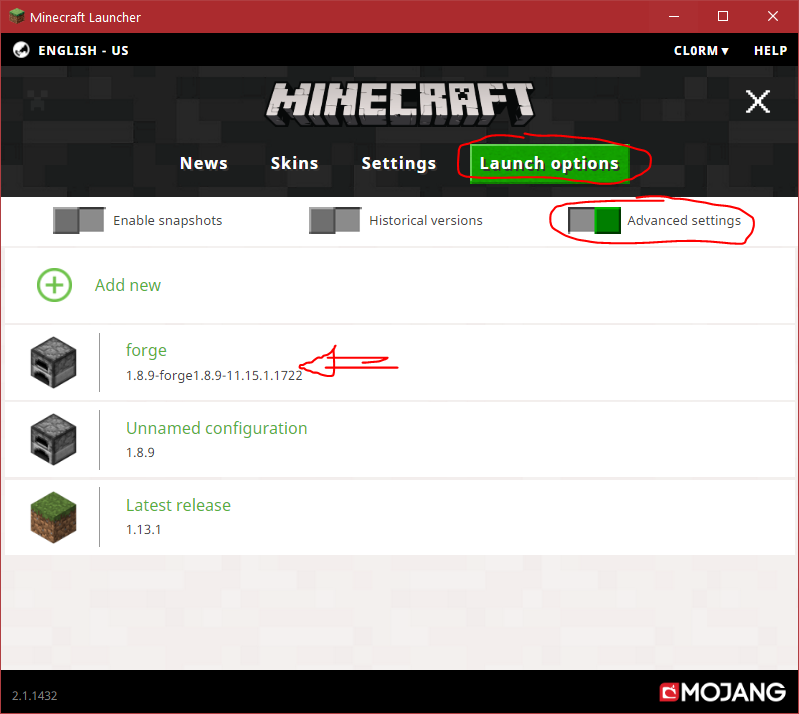
\includegraphics[scale=0.4, center]{TeX_files/pics/installation_1.png}

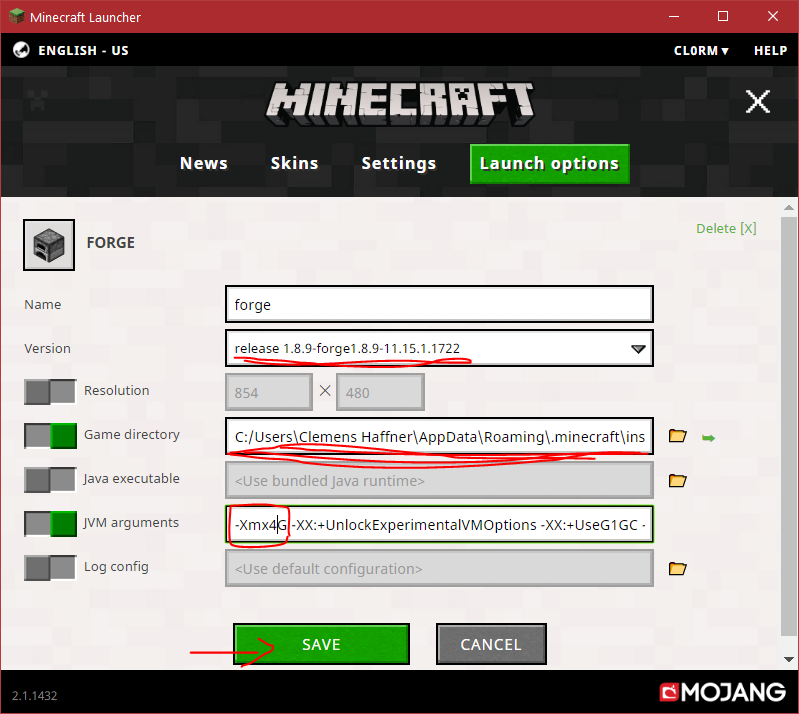
\includegraphics[scale=0.4, center]{TeX_files/pics/installation_advanced_settings.png}

Das Profil startest du einmal, damit Forge die Installation abschließen kann. Bist du im Minecraft-Mainmenu angekommen, kannst du Minecraft wieder schließen.

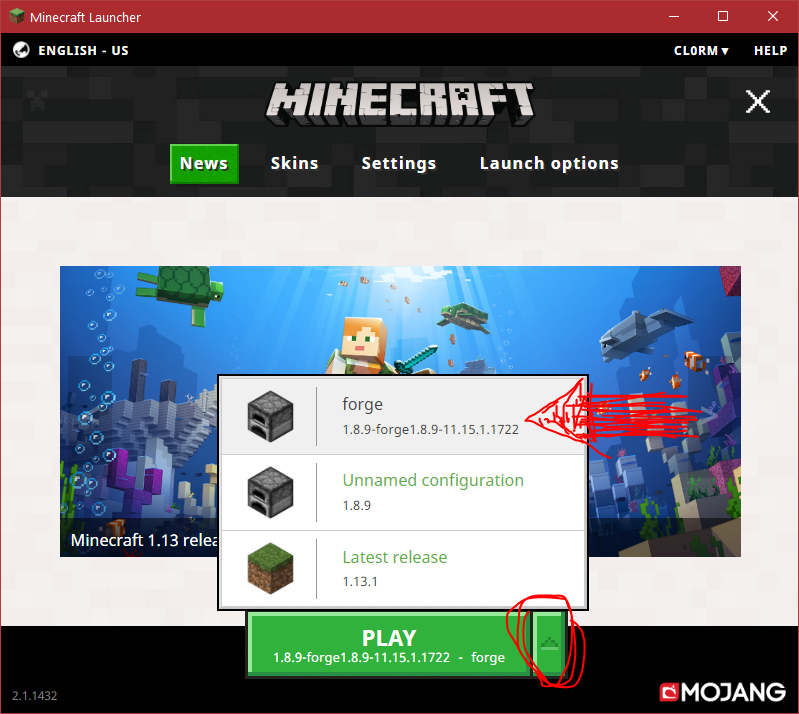
\includegraphics[scale=0.4, center]{TeX_files/pics/installation_starten.png}

Jetzt brauchst du den eigentlichen Hackclient. Dazu besuchst du \url{https://liquidbounce.net/} $\to$ Get Started $\to$ Minecraft-Version auswählen. Die heruntergeladene Datei kopierst du dann in \\ \texttt{\%appdata\%/.minecraft/instances/liquidbounce1.8/mods}
\pagebreak

\section{Der erste Start}
Wenn du jetzt das Minecraft-Profil “forge” startest, solltest du eine neues Mainmenu sehen:

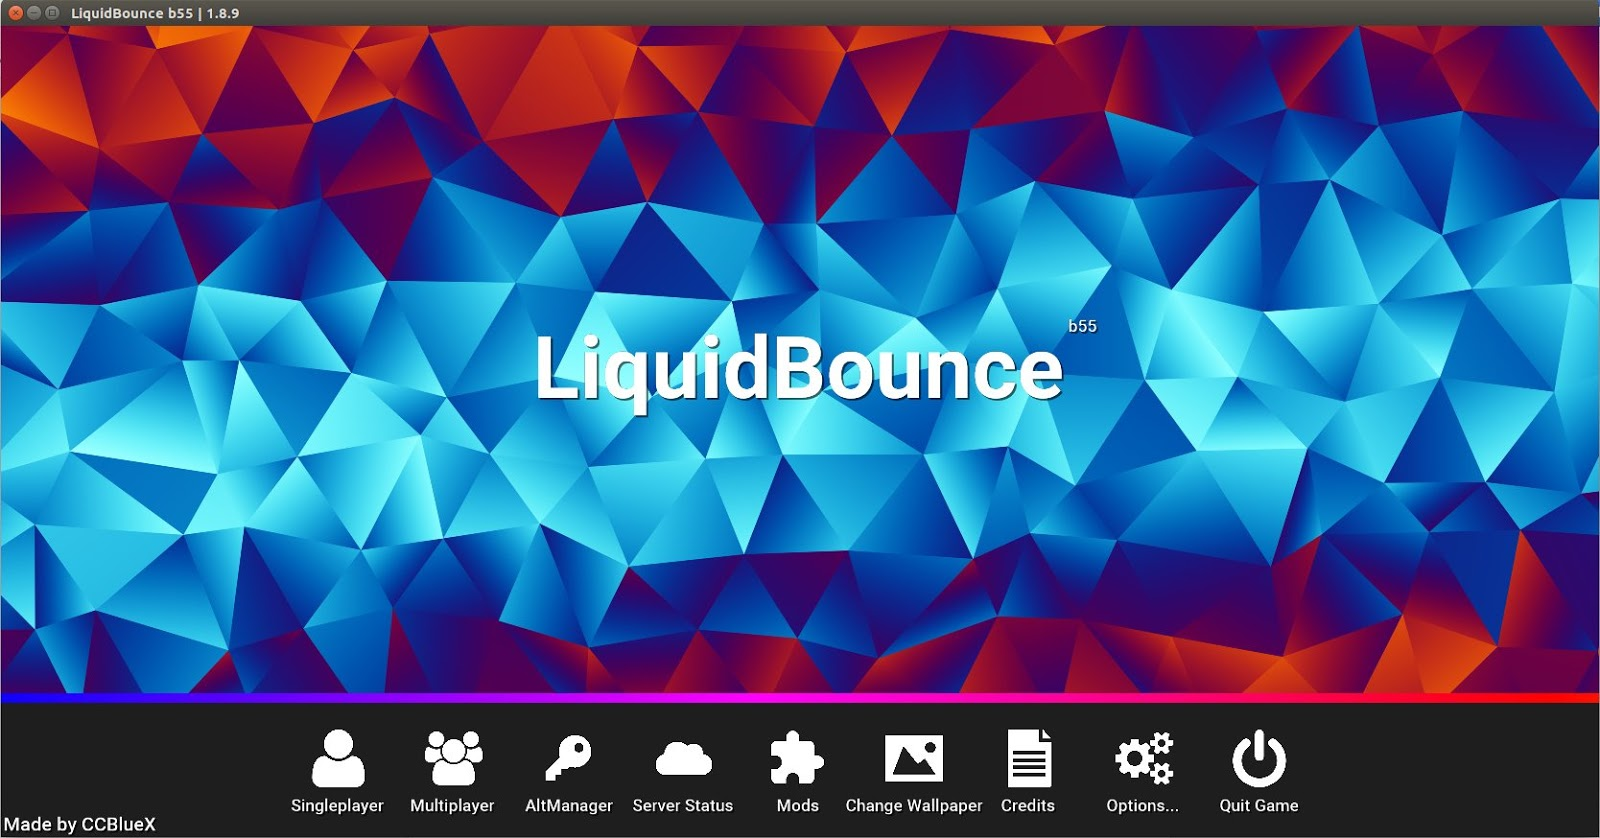
\includegraphics[width=0.7\textwidth, center]{TeX_files/pics/erster_start_1_8.jpg}

Für die Minecraft-Version 1.12.2 sieht das Mainmenu so aus:

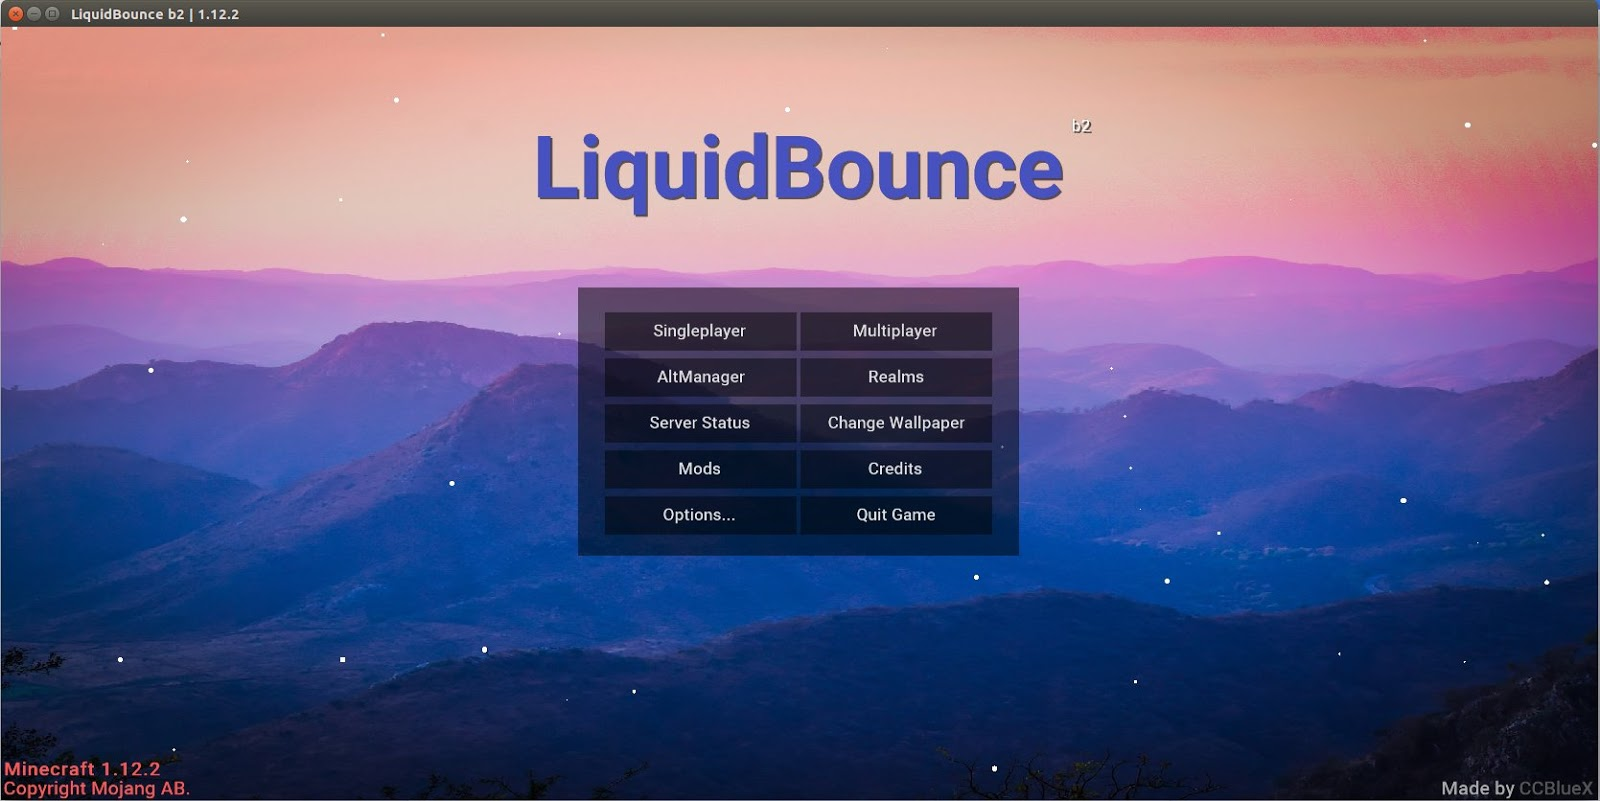
\includegraphics[width=0.7\textwidth, center]{TeX_files/pics/erster_start_1_12.jpg}

Vielleicht kommt noch ein Hinweis, der in wenigen Worten die Handhabung erklärt, aber den kann man auch schnell wegklicken.

Für den Anfang solltest du in eine Singleplayer-Welt gehen und dort alles ausprobieren. Der wichtigste Befehl am Anfang ist: \texttt{.bind clickgui LCONTROL} (Befehle beginnen immer mit einem Punkt und werden ganz normal in den Chat eingegeben, also insbesondere ohne den führenden \texttt{/})

Wenn du jetzt die linke Strg-Taste drückst, öffnet sich das ClickGUI

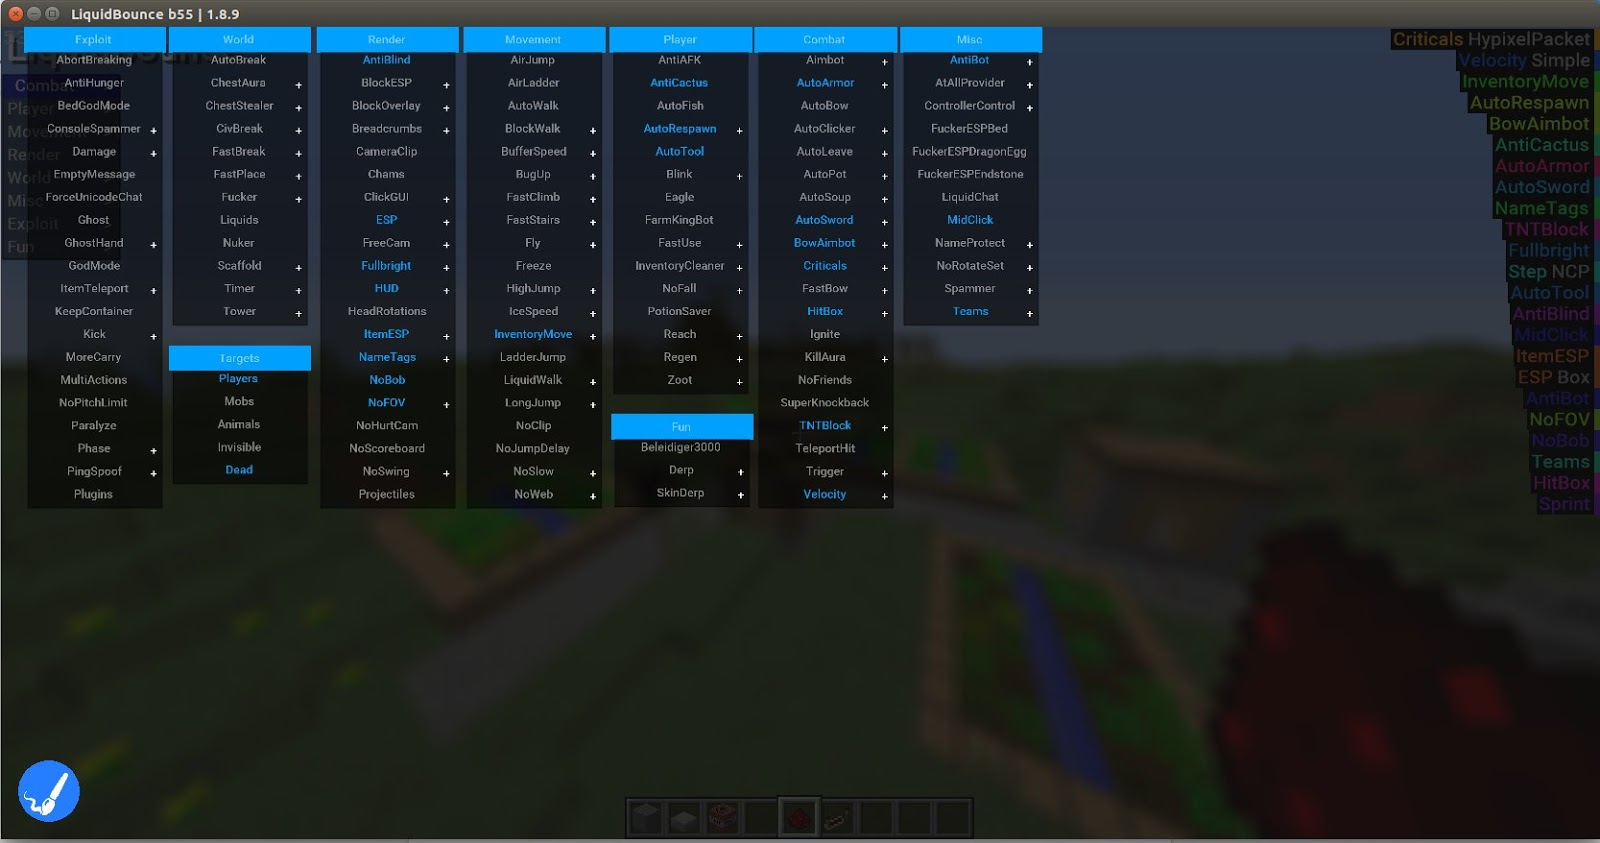
\includegraphics[width=0.7\textwidth, center]{TeX_files/pics/clickgui.jpg}

Die blauen Reiter lassen sich mit Rechtsklick öffnen bzw. schließen und mit gedrückter linker Maustaste bewegen.

Mit dem blauen Pinsel links unten kannst du dein HUD - also zum Beispiel die Liste mit den Hacks, die Anzeige der gerade aktiven Effekte, usw. - verändern. Aber meiner Meinung nach muss man da nichts ändern.

Module (also die Hacks) kann man mit einem einfachen Linksklick aktivieren bzw. auch deaktivieren. Einige Module haben auch weitere Einstellungen, das erkennt man an dem $+$ rechts neben dem Hack. Diese Einstellungen lassen sich mit einem Rechtsklick öffnen und auch wieder schließen. Achtung: In der Regel öffnen sich diese Einstellungen unter den Listen der Reiter, also musst du erst die überdeckende Liste einfahren (Rechtsklick auf den Reiter) und die Einstellungen zu sehen und zu bearbeiten.

\pagebreak

\section{Module}
LiquidBounce hat sehr viele Module und es ist schwer da am Anfang einen Überblick zu bekommen. Ich habe deswegen die wichtigsten Module \textcolor{lime!50}{grün} hinterlegt.

\subsection{Exploit}

Die folgenden Module sind Exploits, die in der Regel auf bestimmten Versionen von Anticheats funktionieren, aber in aller Regel nicht.
\begin{longtable}{p{3cm}|p{10cm}}
\textbf{Hack} & \textbf{Erklärung} \\
\hline
AbortBreaking & Man kann das Abbauen eines Blockes unterbrechen und später weitermachen, ohne seinen Fortschritt zu verlieren. \\
\hline
AntiHunger & Funktioniert manchmal auf alten AAC-Versionen und unterdrückt, dass man Hunger bekommt. \\
\hline
BedGodMode & Funktioniert nur in der 1.9 und ist damit in einem 1.8-Client sinnlos. \\
\hline
ConsoleSpammer & Spammt die Serverkonsole mit Müll zu. Man wird dabei in der Regel gekickt. \\
\hline
Damage & Man fügt sich selber Schaden zu. \\
\hline
EmptyMessage & Sendet eine leere Nachricht im Chat. \\
\hline
ForceUnicodeChat & Ersetzt alle ASCII-Zeichen im Chat durch Unicode-Zeichen. \\
\hline
Ghost & Nachdem man gestorben ist, kann man weiter herumlaufen. Ich sehe keine Verwendung dafür. \\
\hline
GhostHand & Erlaubt es mit Blöcken durch die Wand zu interagieren. Recht nützlich bei Kisten. Man muss den Block, mit dem man interagieren möchte mit \texttt{.ghosthand select chest} einstellen. \\
\hline
GodMode & Ein Exploit für eine alte Version für AAC mit der man nicht sterben konnte. \\
\hline
ItemTeleport & Man kann sich zu Items teleportieren, funktioniert in der Regel nicht. \\
\hline
KeepContainer & Man kann Container (Kisten, Villager-Inventare, ...) von überall öffnen. Noch nie benutzt ... \\
\hline
Kick & Man kann sich selber kicken. Nützlich, wenn man gerade einen Kampf verliert, aber bestraft wird, wenn man den Server verlässt. Ähnliche Funktion wie Damage. \\
\hline
MoreCarry & Man kann in den 4 Crafting-Slots im Inventar Items lagern. \\
\hline
MultiActions & Man kann andere Items benutzen, wenn man gerade Blöcke abbaut. \\
\hline
NoPitchLimit & keine Ahnung ... \\
\hline
Paralyze & Wenn man sich in andere Spieler reinstellt, fängt deren Game an zu laggen. Aber leider auch dein Eigenes ... \\
\hline
Phase & Man kann durch Blöcke laufen. Ähnlich wie NoClip. \\
\hline
PingSpoof & Setzt den vom Server \textit{gesehenen Ping} auf einen festgelegten Wert. Kann nützlich sein, um Items als erster zu bekommen, oder bei manchen Servern Anti-Knockback zu deaktivieren. \\
\hline
\rowcolor{lime!50}Plugins & Zeigt die Plugins an, die auf einem Server installiert sind. Funktioniert recht häufig. \\
\hline
ServerCrasher & Name ist Programm ... Zumindest manchmal. \\
\hline
Teleport & Wenn aktiviert, muss man mit der mittleren Maustaste (in der Regel dem Mausrad) einen Block auswählen. Mit SHIFT teleportiert man sich dann dahin. Nützlich für Jump-and-Runs in Lobbys. \\
\hline
VClip & Teleportiert einen senkrecht nach oben. \\
\hline
VehicleOneHit & Man kann Minecarts mit einem Schlag zerstören. \\
\end{longtable}

\subsection{World}

\begin{longtable}{p{3cm}|p{10cm}}
\textbf{Hack} & \textbf{Erklärung} \\
\hline
AutoBreak & Baut den Block ab, den man gerade ansieht. \\
\hline
\rowcolor{lime!50}ChestAura & Öffnet Kisten in einem Radius. Nützlich in Zusammenhang mit dem ChestStealer. \\
\hline
\rowcolor{lime!50}ChestStealer & Wenn man eine Kiste öffnet, werden alle Inhalte automatisch ins Inventar gezogen, und die Kiste wieder geschlossen. Bei Survival-Games äußerst praktisch. Bitte in Lobbys deaktivieren, da ansonsten deren Menüs buggen. \\
\hline
CivBreak & Baut Blöcke instant ab. Funktioniert in der Regel nicht. \\
\hline
FastBreak & Baut Blöcke schneller ab, sorgt aber in der Regel für Flags, bringt also keinen Geschwindigkeitsvorteil. \\
\hline
FastPlace & Man kann Blöcke deutlich schneller platzieren. Benutzen Legits auch häufig. \\
\hline
\rowcolor{lime!50}Fucker & Zerstört automatisch einen festgelegten Blocktyp in einem Radius um den Spieler (teils auch durch Wände). Macht einen zum Bedwars- / Cakewars-King. Der zu zerstörende Block muss aber mit \texttt{.fucker select bed} eingestellt werden. \\
\hline
Liquids & Erlaubt es einem mit Flüssigkeiten zu interagieren, das heißt auf Wasserquellen Blöcke oder andere Wasserquellen zu setzen. \\
\hline
Nuker & Baut in einem Ring alle Blöcke ab. Vorsicht im Creative-Modus, die Welt ist schnell kaputt. \\
\hline
\rowcolor{lime!50}Scaffold & Setzt Blöcke vor dem Spieler ins Void. Nützlich um sich bei Bedwars rüber zu bauen. \\
\hline
Timer & Beschleunigt die Zeit in Minecraft. Kann als Speed benutzt werden, wird aber häufig erkannt. \\
\hline
\rowcolor{lime!50}Tower & Stackt den Spieler hoch, und zwar extrem schnell. \\
\end{longtable}

\subsection{Targets}

Das sind eigentlich Einstellungen und keine Hacks. Sie beeinflussen, welche Ziele die Killaura angreift und welche Entities im ESP angezeigt werden.

\begin{longtable}{p{3cm}|p{10cm}}
\textbf{Einstellung} & \textbf{Erklärung} \\
\hline
Players & normale Spieler \\
\hline
Mobs & Bösartige Wesen (Zombies, Skeletons etc.) \\
\hline
Animals & Tiere \\
\hline
Invisible & Unsichtbare Wesen / Spieler. \\
\hline
Dead & Tote Spieler / Wesen. Bei einigen Anticheats benötigt, um Spieler korrekt zu erkennen. \\
\end{longtable}

\subsection{Render}

Render-Hacks können von Anticheats nicht erkannt werden. Das ist nur durch Verhaltensanalyse, zum Beispiel bei häufigem schnellen Abbau von Diamanten hintereinander auf Survival-Servers $\to$ X-Ray-Hack.

\begin{longtable}{p{3cm}|p{10cm}}
\textbf{Hack} & \textbf{Erklärung} \\
\hline
\rowcolor{lime!50}AntiBlind & Entfernt den Blindness- und den Nausea-Effekt. \\
\hline
\rowcolor{lime!50}BlockESP & Man sieht den eingestellten Block durch die Wand, zum Beispiel ein Bett bei Bedwars. Muss mit \texttt{.blockesp select bed} konfiguriert werden. \\
\hline
BlockOverlay & Ein anderes Block Overlay. Finde ich hässlich. \\
\hline
Breadcrumbs & Zeichnet eine Linie überall wo man langgeht. \\
\hline
CameraClip & Man kann in der Third-Person-View durch Wände sehen. Man kann aber auch einen ESP benutzen. \\
\hline
Chams & Siehe ESP. Braucht man eigentlich nicht. \\
\hline
\rowcolor{lime!50}ClickGUI & Die Übersicht über alle Hacks. \\
\hline
\rowcolor{lime!50}ESP & Ich kann sehen was du nicht siehst! Durch Wände. Einer der wichtigsten und grundlegendsten Hacks, um sich einen Spielvorteil zu verschaffen. Sollte immer angeschaltet sein. \\
\hline
FreeCam & Ist sie aktiviert, kann man frei herumfliegen mit einer virtuellen Kamera. Man kann also auch sich selbst betrachten. \\
\hline
\rowcolor{lime!50}Fullbright & Man sieht die Welt immer wie am Tag. Sollte immer an sein. \\
\hline
HUD & Damit kann man konfigurieren, welche Elemente man sehen möchte, wenn man nicht in der ClickGUI ist. \\
\hline
HeadRotations & Man sieht die Richtung der Köpfe wie der Server sie sieht. Sinnlos. \\
\hline
\rowcolor{lime!50}ItemESP & Wie ESP, aber für Items. \\
\hline
\rowcolor{lime!50}NameTags & Wichtige Ergänzung für den ESP: Neben den Spielernamen werden Daten dieser Spieler angezeigt wie Leben und Equipment, sowie Rüstung. Macht aber auch die Namen über den Spielern größer und Map-weit sichtbar. \\
\hline
NoBob & Verhindert irgendeinen Clientside-Effekt. Kann man anschalten, muss man nicht. \\
\hline
NoFOV & Verhindert den Zoom-Effekt bei Speed-Potions und beim Sprinten. \\
\hline
NoHurtCam & Bild wackelt nicht, wenn man angegriffen wird. \\
\hline
NoScoreboard & Kein Scoreboard mehr \\
\hline
NoSwing & Keine Swing-Animation des Schwertes. \\
\hline
Projectiles & Man sieht, wo Pfeile, Enderperlen, etc. landen werden. \\
\hline
ProphuntESP & Ein ESP für Versteck-Spielmodi. Funktioniert aber nicht immer richtig. \\
\hline
RemoteView & Erlaubt es das Gesehen durch einen anderen Spieler zu sehen. \texttt{.remoteview Spielername} \\
\hline
\rowcolor{lime!50}StorageESP & Kisten sind durch Wände zu sehen. \\
\hline
SwingAnimation & Eine andere Schwung-Animation des Schwertes. \\
\hline
Tracers & Linien vom Fadenkreuz zu den nächsten Spielern. \\
\hline
TrueSight & Man sieht unsichtbare Entities, wie im Gamemode 3. \\
\hline
\rowcolor{lime!50}XRay & Alle Blöcke außer Erzen, Kisten, etc. sind transparent. \\
\end{longtable}

\subsection{Movement}

\begin{longtable}{p{3cm}|p{10cm}}
\textbf{Hack} & \textbf{Erklärung} \\
\hline
AirJump & Wie ein Double Jump, nur, dass man nicht nur zwei Mal, sondern immer wieder springen kann. Kommt somit einem Fly sehr nahe. \\
\hline
AirLadder & Man kann Leitern hochklettern, ohne sie zu berühren. Hab ichnoch nie benutzt. \\
\hline
AutoWalk & Läuft automatisch in die Richtung, in die man schaut. \\
\hline
BlockWalk & Man kann auf Halfslabs laufen. Noch nie benutzt. \\
\hline
BufferSpeed & Man bekommt auf bestimmten Blöcken einen Speed-Boost. \\
\hline
BugUp & Fällt man im freien Fall (zum Beispiel in Bedwars), so versucht dieser Hack, einen wieder auf einen Block zu teleportieren. Geht eher selten, kann aber nützlich sein. \\
\hline
FastClimb & Leitern schneller hochklettern. \\
\hline
FastStairs & Treppen schneller hochsteigen. \\
\hline
\rowcolor{lime!50}Fly & Durch die Welt fliegen, wie im Creative. Sehr einfach von Moderatoren \textit{und} Anticheat zu erkennen. \\
\hline
Freeze & Man kann in der Luft stehen bleiben. Keine Ahnung wozu das gut sein soll. \\
\hline
HighJump & höher springen \\
\hline
IceSpeed & schneller auf Eis laufen \\
\hline
\rowcolor{lime!50}InventoryMove & Man kann sich mit geöffnetem Inventar (und kann dort sogar sortieren und craften) bewegen. Funktioniert eigentlich immer. \\
\hline
LadderJump & Leitern geben einen Boost nach oben. \\
\hline
LiquidWalk & auch Jesus-Hack. Man läuft auf Wasser und Lava. Manchmal bekommt man sogar keinen Schaden von der Lava. \\
\hline
LongJump & weiter springen \\
\hline
NoClip & Man kann durch Wände laufen. Klappt in der Regel nicht. \\
\hline
NoJumpDelay & Kein Delay beim Springen. Hab da aber keinen Unterschied gespürt. \\
\hline
\rowcolor{lime!50}NoSlow & Man wird nicht durch Blöcke (wie Seelensand) oder Potions verlangsamt. \\
\hline
\rowcolor{lime!50}NoWeb & Wie NoSlow, bei Spinnennetzen \\
\hline
Parkour & Springt an Blockkanten automatisch so weit wie möglich, was bei manchen Jump'n'Runs nützlich ist. \\
\hline
PerfectHorseJump & lässt ein Pferd immer am höchsten springen \\
\hline
ReverseStep & Zieht einen schnell nach unten. Sehr gewöhnungsbedürftig. \\
\hline
SafeWalk & Man muss nicht mehr sneaken, um an Blockkanten nicht mehrrunterzufallen. \\
\hline
SlimeJump & Man springt auf Slime-Blöcken höher. \\
\hline
Sneak & Man sneakt immer. \\
\hline
\rowcolor{lime!50}Speed & Immer am schnellsten unterwegs sein. Verhält sich je nach Modus sehr verschieden, von BHop bis Gleiten ist alles dabei. Ein guter Hacker toggled den Speedhack nur und lässt ihn keinesfalls immer an. Durch Anticheats oft recht einfach zu erkennen. \\
\hline
\rowcolor{lime!50}Sprint & Drückt automatisch Doppel-W. Immer anlassen, außer wenn man hierdurch zu viel Essen verliert. Klappt auf manchen Servern auch rückwärts. \\
\hline
\rowcolor{lime!50}Step & Springt an Blockkanten automatisch hoch, teleportiert dich aber in der Regel den Block hoch. Bei manchen Servern sogar an Kanten, welche für Legits zu hoch sind (1,5 - 2 Blöcke hoch). \\
\hline
Strafe & Man kann extremer Strafen im Sprung (also zum Beispiel einen 360 machen, Projektilen ausweichen) \\
\hline
WallClimb & Wände hochklettern, wie wenn Leitern daran wären. \\
\hline
WallGlide & Man kann an Wänden gleiten. \\
\hline
WaterFly & Wie fliegen, aber nur unter Wasser. \\
\hline
WaterSpeed & Schneller im Wasser unterwegs sein. \\
\end{longtable}

\subsection{Player}

\subsection{Fun}

\subsection{Combat}

\subsection{Misc}
\pagebreak

\section{Befehle}
Befehle beginnen in LiquidBounce mit einem Punkt \texttt{.}. Damit kann mal alle Einstellungen der Module auch ohne die ClickGUI machen. Benutzt wird dieses Feature unter anderem für die Autosettings - damit wird der Client gleich mit den passenden Bypasses für den Server ausgerüstet.

Um die Autosettings eines Servers zu laden, gibt man in de Chat ein: \texttt{.settings load gomme}. Autosettings sind für viele Server verfügbar, eine Liste bekommt man mit \texttt{.settings list} oder man schaut einfach auf der Github-Seite des Entwicklerteams nach: \url{https://github.com/CCBlueX/FileCloud/tree/master/LiquidBounce/autosettings}

Weitere nützliche Befehle:
\begin{itemize}
    \item \texttt{.bind Modulname KEY} - Hotkeys für Module festlegen
    \item \texttt{.friends [add/list/remove] Name} - Friendlist verwalten
    \item \texttt{.localsettings [save/list/load] Name} - Eigene Settings abspeichern
    \item \texttt{.serverinfo} - Infos über aktuellen Server
    \item \texttt{.help} - Zeigt Hilfe an
\end{itemize}
\pagebreak

\section{Alts}
Alts steht für \textit{alternative Accounts}. In LiquidBounce gibt es einen recht komfortablen Manager, mit dem man seinen Account wechseln kann, ohne dabei Minecraft neu starten zu müssen.

Man kann sich alternative Accounts im Internet besorgen, Quellen für Alts sind z.B.
\begin{itemize}
    \item FreeGG (nicht zu empfehlen, sehr aufwendig)
    \item Cracker / WareZ / Hacking - Foren (recht gute Ausbeute)
    \item YouTube-Videos (funktionieren aber sehr schlecht)
\end{itemize}

Um die Accounts auf ihre Funktionsfähigkeit zu überprüfen, sollte man beachten, dass das schnelle Ausprobieren von Accounts hintereinander von der selben IP von Mojang schnell mit einem IP-Ban bestraft wird. In diesem Fall heißt es etwa 30 Minuten (?) warten. Es gibt im Internet viele Account-Checker, die diesen Auftrag für einen übernehmen (siehe zum Beispiel \url{https://www.nulled.to} für Alt-Checker). Die meisten Checker kosten allerdings Geld, gecrackte Versionen können allerdings Malware enthalten oder die funktionierenden Accounts an den Entwickler heimlich weiterreichen. Überprüfung mittels Virustotal\footnote{\url{https://www.virustotal.com/\#/home/upload}} auf Viren und Überwachung des Netzwerktraffics mittels Wireshark \footnote{\url{https://www.wireshark.org}} wird empfohlen.

Mit entsprechenden Skripting-Kenntnissen kann man sich aber auch seinen eigenen Account-Checker bauen. Für Linux-User ist folgendes Github-Repository (\url{https://github.com/air/minecraft-tools}) ein guter Anlaufpunkt.

\textbf{ACHTUNG:} Die meisten Alts, die man im Internet bekommt, sind gekaperte / gehackte Minecraft-Konten. Man muss sich beim verwenden solcher Accounts bewusst sein, dass man damit das Geschäft mit gecrackten Accounts ankurbelt. Während hacken in Spielen völlig legal ist (wenn auch unerwünscht von Einigen), sind Alts daher je nach Quelle entweder als Grauzone oder als illegal einzustufen.
\pagebreak

\section{gute Server und Spielmodi zum hacken}
\begin{longtable}{p{4cm}|p{4cm}|p{4cm}}
    \textbf{Server} & \textbf{Spielmodi} & \textbf{Bemerkungen} \\
    \hline
    Minesucht & KnockFFA & Legits regen sich immer lustig auf, Mods sehr inaktiv. Anticheat ist nach Update mittlerweile recht gut geworden. Hab noch keine guten Autosettings gefunden. Anticheat verteilt IP + Username-Bans. \\
    \hline
    Mineplex & Sehr viele, hauptsächlich Cakewars, Survival Games & eher den US-Server nutzen (us.mineplex.com), da dort mehr Leute on sind. Recht gnädiges Anticheat, dafür, dass es einer der größten Server ist. Modbans allerdings häufiger. Meist 30-Tage-Bans \\
    \hline
    Hypixel & alle Spielmodi, mein persönlicher Favorit ist VampireZ & es funktionieren nur wenige Alts, dafür aber so gut wie keine anderen Hacker verteilt meist Permabans, Runden werden schnell voll \\
    \hline
    CubeCraftGames & SkyPVP & starke Killaura, Runden werden schnell voll \\
    \hline
    GommeHD & GunGames, Bedwars, Skywars & Sehr wenige funktionierende Alts, nur Permabans, man wird meist recht schnell gebannt. Spielspaß aber garantiert, inklusive wütender Legits. \\
    \hline
    HiveMC & Bedwars & Runden werden relativ schnell voll, Anticheat bannt nicht, Mods inaktiv, Killaura verhältnismäßig schwach, das heißt man braucht schon etwas Equipment, um gegen Legit-Teams anzukommen. Fucker geht aber durch Wände! \\
    \hline
    MC-Central & viele, hauptsächlich Cakewars & Meist 30-Tage-Bans. Alts meist nicht gebannt, starkes Anticheat, aber sehr gute Killaura. Runden füllen sich nur träge.
\end{longtable}

\end{document}
